%Réalisation technique
    %Contexte technique opérationnel
        %Plan de vol et reports ADSC
        %Plate-forme TIARE (production de log fichiers texte)
    %Base de travail
        %Python : librairies, IDE, Linux
        %Google Earth
    %Conception Produit
            %Le programme réalisé et ses fonctions
                %Analyse DATASET
                %Analyse du trafic
    %Problèmes techniques rencontrés
            %Rotondité, intersection, zip, optimisation dans google earth….



%Avant de passer à la pratique un apprentissage théorique à du être réalisé.
\section{Architecture du logiciel}
    \subsection{L'interface \textsc{Google Erath}}
\textsc{Google Earth} dispose d’une interface graphique qui sera mise à profit pour:
\begin{itemize}
\item représenter les points remarquables (points nommés, points de coordination, etc.),
\item représenter les espaces de contrôle,
\item représenter le trafic aérien.
\end{itemize}\medskip

Ces données sont, soit statiques, soit dynamiques.
\begin{description}
\item[Statiques:] affichage de points fixes et affichage des espaces ou trajectoire plan de vol. 
\item[Dynamique:] représentation du trafic aérien en fonction de coordonnées mises à jour et en fonction du temps.
\end{description}\medskip

    \subsection{Gestion de l'affichage}
Google Earth peut être enrichi de données externes via un fichier descriptif de données (\textsc{Kmz}).

Ce fichier Kmz n'est autre qu'un fichier Zip compriment un fichier "doc.kml" ainsi que les fichiers vers les quel il pointe. Ce fichier "doc.kml" a pour but de regrouper les fichier à ouvrir (comme le ferait une liste de lecture pour les fichiers Mp3). Il indique donc à \textsc{Google Earth} de charger les fichiers suivant:
\begin{description}
\item[CharacteristicsPoints.kml:] Le fichier contenant les points remarquables
\item[Fir.kml:] pour les zones de contrôle et la zone \textsc{Aci} 
\item[Routes.kml:] regroupe toutes les routes définies
\item[Fpl.kml:] affiche les plans de vol déposés
\item[Ads.kml:] affiche le trafic aérien réel recu par l'\textsc{Adsc}
\end{description}\medskip

Les fichier KML sont fabriqués à partir des fichiers de configuration et de traces définis dans le système EurocatX. 

Le système EurocatX est configuré au moyen de fichiers de configuration statique. Ces fichiers seront «parsés» pour fabriquer les fichiers: "CharacteristicsPoints.kml", "Fir.kml" et "Ads.kml".

Ce système est également constitué de fichiers de traces qui log les informations de vol. Ces fichiers seront «parsés» pour fabriquer les fichiers: "Ads.kml" et "Fpl.kml".

    \subsection{Les modules}
Au final le logiciel se compose des modules suivants:
\begin{description}
\item[Manu:] Fichier principal, peut être considéré comme l'exécuteur. \nref{pyManu}
\item[modules/Ads:] Met en mémoire les information sur les report \textsc{Ads}. \nref{pyAds}
\item[modules/Aoi:] Permet de définir tout les volume utilisé pour concevoir les zone de contrôles. \nref{pyAoi}
\item[modules/CharacteristicPoints:] Met en mémoire tous les points remarquables disponible sur le système. \nref{pyCP}
\item[modules/Convertion:] Regroupe plusieurs fonctions utiliser pour convertir des donnée (ex: utilisé pour convertir les coordonnées). \nref{pyConvertion}
\item[modules/Fdp:] définit et met en mémoire toutes les zone de contrôles. \nref{pyFdp}
\item[modules/Fpl:] définit et mets en mémoire les plans de vol. \nref{pyFpl}
\item[modues/GetOfFiles:] Coordonne la récupération des donnée, c'est lui qui va chercher la configuration et lance les modules tel que Aoi, Fdp ou encore Fpl. \nref{pyGOF}
\item[modules/KML:] Ce module est utilisé pour mettre en forme les fichier \textsc{Kml} à l'aide des données reçues en entrée (par exemple pour un point il reçois ça description, ces coordonnées, son nom ...). \nref{pyKML}
\item[modules/MakeKML:] C'est le module qui exploite toutes les données en mémoire et crée les fichiers \textsc{Kml}. \nref{pyMakeKML}
\item[modules/MakeKMZ:] Récupère les fichiers \textsc{Kml} pour les regrouper en un fichier \textsc{Kmz} plus maniable. \nref{pyMakeKMZ}
\item[modules/Routes:] définit et mets en mémoire les routes definies. \nref{pyRoutes}
\item[modules/usualFonction:] Regroupe plusieurs fonction régulièrement utilisées. \nref{pyusualFonction}
\end{description}
Chaque module est décrit avec plus de précisions en annexe.

Le fichier principal (Manu.py) se lance à partir de la ligne de commande: "Python~Manu.py" dans un système ou Python est installé et correctement configuré.

Les fichiers ".asf" contenant la configuration de l’eurocatx sont placés dans le répertoire "SurcesAsf" alors que les fichiers contenant les traces sont dans le répertoire "Sources". 

Tout les modules sont appelé automatiquement, se qui signifie qu'une foi le fichier de configuration renseigner et le fichier principal lancé, aucune action n'est nécessaire jusqu'a la réception du fichier \textsc{Kmz}. Il n'y aura donc plus qu'a lancer se fichier en l'ouvrant depuis \textsc{Google Earth}. 

\section{Le contexte technique opérationnel}

    \subsection{\textsc{EurocatX}}
Il faut bien comprendre comment marche le système afin de bien visualiser d'où proviennent les informations. Comme décrit grossièrement dans le schéma (cf. Fig. \vref{eurocatx}),
\begin{figure}[!h]
    \center
    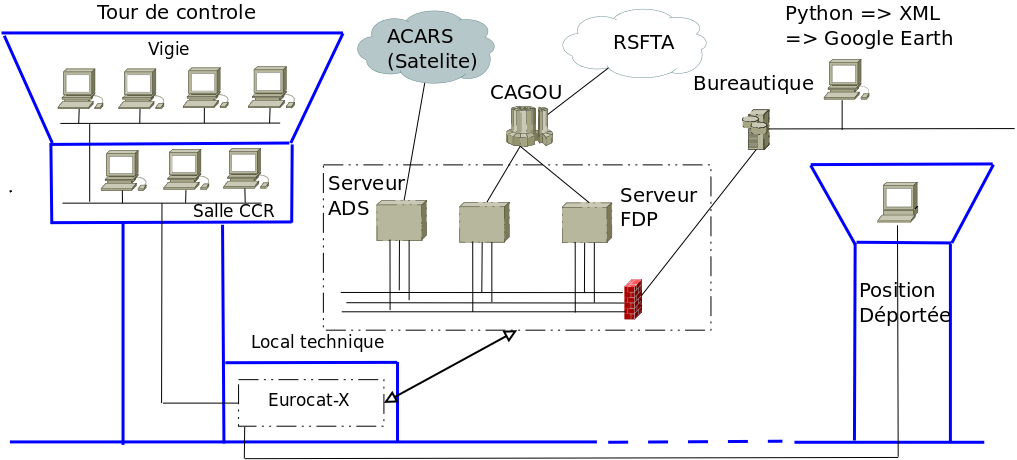
\includegraphics[width=15cm]{images/SchemaControle.png}
    \caption{Schématisation du système \textsc{EurocatX} au niveau des tours de contrôle}
    \label{eurocatx}
\end{figure}
\textsc{EurocatX} récupère les informations sur les plans de vol par l'intermédiaire de \textsc{Cagou}\footnote{\textsc{Cagou}: nom donné au commutateur \textsc{Rsfta}}. Il récupère aussi le positionnement émis par l'avion à l'aide de la transmission Satellite, \textsc{Vhf}\footnote{\textsc{Vhf}: Very High Frequency, soit une bande radio de très haute fréquence} ou des données radars lors de son approche. Le système \textsc{EurocatX} donne un accès à la bureautique protégé par un par-feu (FireWall) afin de rendre disponible sur ce réseau un certain nombre d'information. Dans notre cas nous y récupérerons:
\begin{itemize}
    \item toutes les données de configuration du système tels que les nom et coordonnées des balise référencée, la position des zone de contrôle et des zone \textsc{Aci} ou encore les route utilisée pour décrire les plans de vols.
    \item Les fichiers de log du Commutateur \textsc{Cagou} afin de pouvoir exploiter les plans de vol reçus par le réseau \textsc{Rsfta}.
    \item Tous les reports \textsc{Ads} reçu par satellite et traité par le système.
\end{itemize}\medskip 
Le système envoyé les informations récoltées et celle calculées au visues\footnote{Visue: Nom pour décrire les ordinateur utilisés pour visualiser les données de contrôles} situées dans la tour de contrôle au niveau de la Vigie ou de la salle \textsc{Ccr} ainsi que de la position déportée à \textsc{Morea}.

Les données seront donc récupérée dans les fichiers ".asf" pour tous ce qui est de la configuration du système, dans les fichier du \textsc{Fdp} pour les plans de vol et dans les fichiers du serveur \textsc{Ads} pour les reports ainsi que pour la position calculée des aéronefs.

    \subsection{Le domaine de l'aviation}
Il m'a aussi été nécessaire de prendre connaissance de touts les termes, unité, convention et j'en passe utilisé dans le domaine aéronautique.

        \subsubsection{Les coordonnées et unités:}
Tout d'abord est vite venu le problème de conversion de coordonnées, J'ai donc du revoir les conversions de coordonnées sphériques ainsi que les conversions de distances.
J'ai également du, comme expliquée ci dessous (cf. \vref{mathcoord})
me remémoré les solutions de calcule du point d'intersection de deux arc de cercle en coordonnées sphériques.

        \subsubsection{Convention:}
Plusieurs conventions on du être acquise comme celle utilisé par le système TIARE pour décrire les report \textsc{Ads} ou encre celle utilisée par les compagnies pour le dépôt de plan de vole.
NE PAS OUBLIER DE FAIRE RÉF AU DOCUMENT 4444 ...





\section{Base de travail}
    \subsection{Le langage Python}
        \subsubsection{Bien coder:\label{pygood}}
Afin de pouvoir apprendre les bonne pratique de la programmation Python j'ai lu un livre intitulé "Programmation Python, conception et Optimisation"\cite{pybook}. Celui-ci m'a permit de pouvoir d'une part revoir ce qui avait été appliquer lors de mes études et d'autre part avoir une vue global sur le langage et ainsi pouvoir prendre du recule lors du codage.

Celui ci m'a par exemple appris le nouveau style de programmation qui part du principe que chaque nouvel objet définit est basé sur un Objet existant, et que par la même occasion tout en python était Objet (même une simple variable booléenne). Ou encore la manière de vérifier si un objet était faux, égale à 0 ou encore une chaîne vide simplement en demandant si il existait (ex:~\texttt{"if x != 0:"}~devient \texttt{"if not x:"})

        \subsubsection{Utiliser les expressions régulières:} 
L'apprentissage de l'utilisation des expressions régulières\footnote{Une expression régulière est en informatique une chaîne de caractères que l’on appelle parfois un motif et qui décrit un ensemble de chaînes de caractères possibles selon une syntaxe précise.}, m'a été grandement facilité garce au site: \url{http://www.dsimb.inserm.fr/}\cite{re} et a la documentation en ligne de Python\cite{pydoc}. Il s'est avéré après apprentissage que ces expression régulière aurons grandement facilité la faisabilité du projet.

        \subsubsection{L'optimisation:}
Je pourrais cité un passage du livre\cite{pybook} qui dit:
\begin{quotation}
    Fourni dès le départ avec des modules de tests, Python est un langage agile. Le terme agile est originellement issu de la méthodologie de programmation agile (Beck et Al.), très proche de la programmation itérative. Cette méthodologie, qui réduit les risques liés à la conception de logiciels, introduit entre autres des principes de tests continus du code.
    \raggedleft Vincent \textsc{Lozano}.
\end{quotation}

En effet il m'a été rapidement nécessaire de réalisé des test, aussi bien pour vérifier que mon code était valide que pour vérifier que celui-ci s’exécutait normalement. Il c'est avéré à plusieurs reprises que certaines parties de mon code étaient très gourmandes en processus. L’apprentissage de fonctions de test de code, tel que le module hotshot décrit plus tard (cf. \vref{perf}), m'a été rapidement nécessaire.

    \subsection{\textsc{Google Earth}}
\textsc{Google Earth} est un logiciel, propriété de la société \textsc{Google}, permettant une visualisation de la terre en 3 dimensions avec un assemblage de photographies aériennes ou satellites. Ce logiciel donne la possibilité de configurer un environnement, ajouter des lignes, des points ou encore des polygone en 3D en passent par des fichier de configuration au format KML\footnote{\label{Kml}KML: Keyhole Markup Language, est un format de fichier et de grammaire XML pour la modélisation et le stockage de caractéristiques géographiques comme les points, les lignes, les images, les polygones et les modèles pour l'affichage dans \textsc{Google Earth}, dans \textsc{Google Maps} et dans d'autres applications.}.

Ce format, qui repose sur le XML\footnote{XML: Extensible Markup Language («langage extensible de balisage»), est un langage informatique de balisage générique.}, a l'avantage d’être simple à manipuler. Ça sémantique est définie sur le de google (cf. Bibliographie \cite{gecode}) 



\section{Le programme réalisé et ses fonctions}
    \subsection{Le fonctionnement\label{fonctionnement}}
            \paragraph{La configuration:}
Le programme réalisé ne possède pas encore d'interface (IHM) graphique. Il est donc nécessaire de configurer les option a l'aide d'un fichier de configuration (cf. annexe \vref{config}). Nous pourrons régler par l'intermédiaire de celui-ci:
\begin{itemize}
    \item Les fichiers Kml à recréer ou non, se qui est utile afin de ne pas avoir à recréer des fichiers statique (tel que la position des point caractéristique ou encore des zones de contrôles) a chaque utilisation tout en laissant a l'utilisateur la possibilité de les mettre a jour simplement.
    \item Les différant styles et couleurs.
    \item L'emplacement des fichiers de configuration.
    \item les description et noms appliqué à chaque catégorie.
\end{itemize}\medskip
            \paragraph{L'exécution:}
Le fichier de configuration renseigné, le programme peut être lancé. Il est possible de le lancer par l'intermédiaire d'un Shell\footnote{Shell: Interface en lignes de commandes}, par l'intermédiaire de l'interface Python ou encore en direct si les informations pour gérer et lancer les fichiers Python ont été renseignées dans le système d'exploitation.
            \paragraph{Le résultat:}
L'exécution du programme réalise une suite d'action:
\begin{enumerate}
    \item Lire le fichier de configuration afin de déterminer les action à effectuer.
    \item Lire les fichiers de configuration du système \textsc{Tiare} affin de récupérer toutes les variable nécessaire sous forme d'objet\footnote{Objet: structure de données valuées et cachées qui répond à un ensemble de messages. Cette structure de données définit son état tandis que l'ensemble des messages qu'il comprend décrit son comportement} (ex: points caractéristique ...)
    \item Lire les fichiers de log afin de créer des objets tel que les plans de vol ou encore les reports \textsc{Ads}. Ces objet sont créer non seulement a partir de ses fichiers de log mais aussi a partir des objets créer précédemment (ex: les point des plan de vol désigné par un nom sont convertis en coordonnées à l'aide des points caractéristiques).
    \item Créer les fichiers \textsc{Kml} désigné dans le fichier de configuration à l'aide des objets instancié.
    \item Créer un fichier \textsc{Kmz} a l'aide de tout les fichiers \textsc{Kml} afin d'avoir un fichier compact et facile a transporter.
\end{enumerate}

    \subsection{L'exploitation dans \textsc{Google Earth}}
L'execution du programme retourne en résultat un fichiers \textsc{Kmz}. C'est ce fichier qui est utiliser pour éxploiter les données dans \textsc{Google Earth}. Pour cela il suffit d'ouvrir le fichier à l'aide de ce logiciel.

Nous allons vous présenter quelques exemple d'utilisation de ce logiciel.

        \subsubsection{Vue d'ensemble}
\begin{figure}[!h]
\center
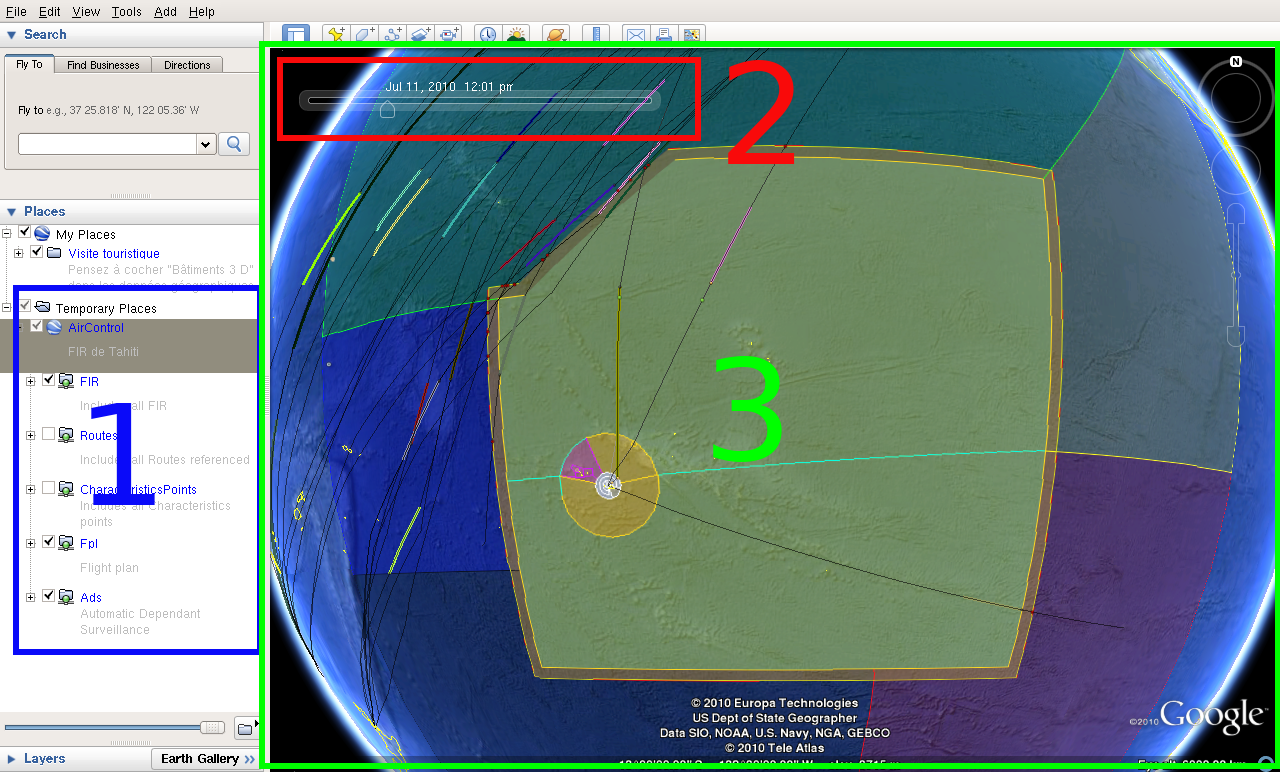
\includegraphics[width=12cm]{images/gevuedensemble.png}
\caption{Vue d’ensemble du trafic dans \textsc{Google Earth}}
\label{gevuedensemble}
\end{figure}
Lors de l'ouverture du fichier la vu est centrée sur la zone de contrôle de Tahiti. Comme vous pouvez le voir \figref{gevuedensemble} nous pouvons distinguer trois zones dans le logiciel:
            \paragraph{La zone de sélection :}
Cette zone, numéroté 1 sur la figure, sert à sélectionner les éléments à afficher ou non. 

Chaque groupe d'éléments est représenté par un dossiers. Ainsi il serra plus facile de sélectionner un groupe tel que les routes. Il sera aussi simple de dé-sélectionner un groupe (par exemple groupe Fpl qui contient tout les plans de vol) et de re-sélectionner un seul élément du groupe afin de le visualiser séparément (ex: le plan de vol d'un avion précis).

            \paragraph{L'animation temporelle:}
Sur notre figure cet outil est représenté par le numéro 2. Nous pourrons grâce a lui visualiser l'évolution du trafic dans le temps. Les principale option utile a notre cas seront:
\begin{itemize}
\item La sélection d'une date et une heure précise afin de visualiser ou devrait se trouver un avion ou encore avoir une vue de tout les vole en cours à cette heure.
\item Un créneau compris entre deux date et heure. Cette option nous permettra de visualiser un vol sur un partie de son parcours afin d'avoir une vue un peut plus globale. Nous l'avons utilisé lors de l'exemple suivant \figref{gezoom} afin de mieux visualiser les points estimé par le système \textsc{Tiare}.
\end{itemize}

            \paragraph{La vue:}
Cette zone, numérotée 3, nous permet visualisée notre sélection configurée à l'aide des deux zones citées précédemment.

        \subsubsection{Exploitation des données}
\begin{figure}[!h]
\center
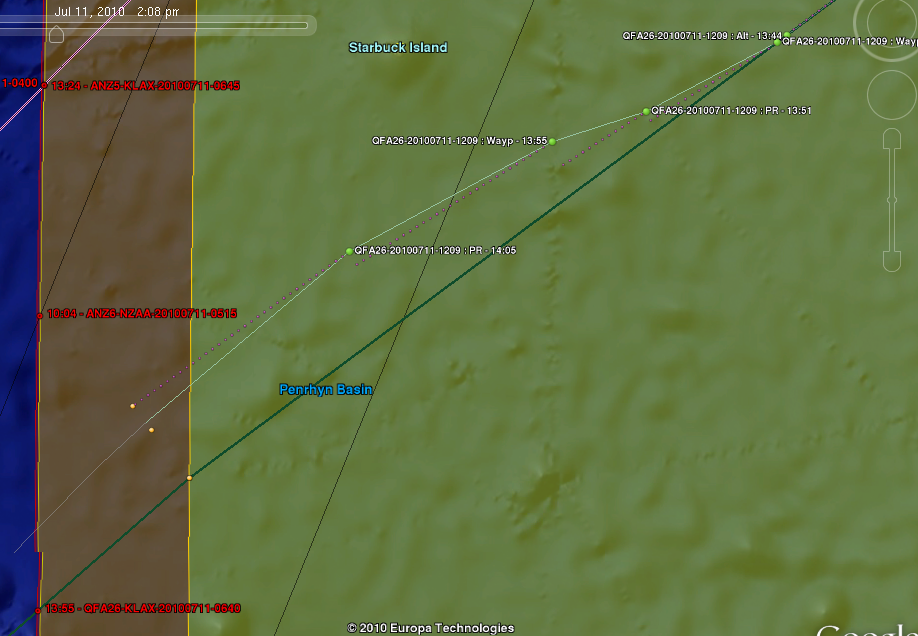
\includegraphics[width=12cm]{images/gezoom.png}
\caption{Zoom su la déviation de la trajectoire d'un vol par rapport a son plan de vol déposé}
\label{gezoom}
\end{figure}
Nous avons pris en exemple un zoom sur un plan de vol qui a été dévié de son sa trajectoire initiale (son plan de vol).
Nous pouvons donc apercevoir sur cette figure \figref{gezoom}:
\begin{description}
\item[Les lignes noires] Ces ligne représente les plans de vol des avions en cours a la date et l'heure sélectionnée. Ci ceux-ci ne sont pas recouvert par une ligne de couleur plus épaisse, cela signifie que l'avion n'est pas censé se trouver a cet endroit a l'instant défini. 
\item[La ligne verte:] Cette ligne représente le plan de vol déposé. Chaque segment de cette ligne représente ou peut se situer l'avion a l'instant donné.
\item[La ligne blanche:] Cette ligne représente la trajectoire réellement effectuée par l'avion. Cette ligne est définie par les report \textsc{Ads}.
\item[Les points verts:] Ces points représente les report \textsc{Ads} reçu par le système \textsc{Tiare}. Lorsque l'on clic sur l'un de ces point il est possible de voir ça description qui contient le message émis par l'avion pour définir ce point.
\item[Les points roses:] Ils représentent les points estimés par le système \textsc{Tiare}. Dans ce cas précis nous constatons que ces points ne correspondent pas avec la trajectoire réellement réalisée. Cette différence peut s'expliquer par le fait que le système utilise les point de reports suivant estimé par l'avion pour définir la position actuel de l'avion.
\item[Les points oranges:] Ces point représentent les reports suivant estimés (next report) par l'avion cité précédemment.
\item[Les points rouges:] Ces points représente l'heure d'entrée, estimé par le programme, dans la zone \textsc{Aci} \nref{Aci}. 
\end{description}




\section{Problèmes techniques rencontrés et solution apportées}
Comme dans tout projet il y a une multitude de problèmes à résoudre. Nous verrons dans cette partie quelques exemples de ces problèmes rencontrés ainsi que la manière dont ils ont été résolus. Cette liste reste bien entendu exhaustive au regard de tous les petits problèmes auxquels nous avons du faire face.

    \subsection{Gestion des erreurs}
            \paragraph{Problématique:}
Le premier problème que nous avons rencontré a été celui de la gestion des erreurs. En effet, de la première mise en route du logiciel jusqu'à la fin du stage des erreurs ont du être gérées. Deux types d'erreurs sont revenues:
\begin{itemize}
    \item Le premier type d'erreur était par exemple une réaction in attendue du logiciel, On pourrait prendre en exemple la conversion de coordonnées reçue en Système sexagésimal \footnote{(Système sexagésimal : Degrés ( \degres\ ) Minutes ( ' ) Secondes ('' ))} en coordonnées décimales utilisées dans les fichiers KML \vref{Kml}, qui lors des premiers tests donnait des donnée erronées.
    \item Le deuxième type était celui du aux erreurs contenues dans les fichiers de log utilisés pour récupérer les informations. Ces erreur faisaient effet boule de neige et venait se répercuter dans le fonctionnement du logiciel.
\end{itemize}\medskip

            \paragraph{Résolution:}
La solution au premier problème a été de mettre en place des test a chaque fonction implémenter ou après avoir réaliser chaque objectif fixé. On appel cette méthode le test continu du code. Grâce à cela nous allons pouvoir déterminer plus rapidement lors d'une erreur futur d'où provient celle-ci. Une méthode simple de la mette en place est de définir un test a réaliser pour valider la fonction ou le code. On détermine donc quel réaction doit avoir un fonction pour un environnement donné et l'on vérifie si le résultat corresponds bien avec celui espéré. (Ex: on a la coordonnée 4530N10045E qui correspond a 45\degres 30' Nord 100\degres 45' Est. On envoi cette variable dans la fonction de conversion et l'on vérifie que le résultat retourné est bien en décimal: 45,5\degres\ en latitude et -100,75 en longitude). Si le résultat est correct la fonction ou le morceau de code est validé, sinon il doit être corrigé.

La solution du deuxième problème a été dans un premier temps d'afficher chaque erreur dans la console, mais cela est vite devenu trop compliqué du fait que la console ne retient par défaut qu'un nombre limité de ligne en mémoire et que les ligne trop ancienne sont simplement effacée. On a donc mis en place un système de log permettant, en plus d'avoir accès au information les plus ancienne, de pouvoir l'exploiter ares avoir fermé la console, effectuer des recherche a l'intérieur et tout avantage que peut apporter un fichier texte. Pour les dernière version de log, celles-ci sont crées avec des information relative au type d'erreur et l'emplacement de l'erreur dans le fichier source, le tout enregistrées dans un fichier comprenant la date et l'heure actuel dans le nom afin de pouvoir les différencier de chaque exécution du logiciel. 

    \subsection{Intersection entre plans de vol et zone ACI\label{mathcoord}}
            \paragraph{Problématique:}
Afin de déterminer l'heure d'entrée approximative des avions dans la zone ACI (cf. \vref{Aci}) en fonction de leur plan de vol déposé Il est nécessaire de déterminer le point d'intersection entre leur plan de vol et la zone ACI. En théorie cela paraît simple, il suffit de prendre chaque portion du trajet du plan de vol composé de deux point et formant une droite, et  de déterminer si cette droite coupe chaque droite composant la zone ACI. Dans la pratique il c'est avéré que cela était un peu plus compliqué, en effet ces droites sont en réalité des arcs de cercles qui sont composé de deux extrémités définies par des points en coordonnées sphériques (cf. schéma fig. \vref{sphere}).
\begin{figure}
    \center
    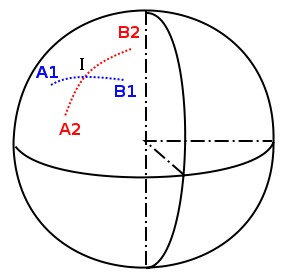
\includegraphics[width=5cm]{images/Sphere.png}
    \caption{Représentation grossière de l'intersection de deux arc de cercle respectivement formé par la trajectoire la plus courte entre deux points situé sur le Globe terrestre}
    \label{sphere}
\end{figure}
            \paragraph{Résolution:}
Étant donné que j'ai effectué un BTS avant d'intégrer l'EIGSI \footnote{EIGSI: École d'Ingénieurs en Génie des Systèmes Industriel située à La Rochelle}, les notion de coordonnées sphérique ne me sont que peut familière. Après avoir en vainc cherché sur internet ainsi que dans mon entourage  (maître de stage, collègues de travail) je me suis replié sur un forum de mathématique sur le quel j'ai déposé un sujet explicitant le problème (adresse, cf. bibliographie \cite{forummath}). Une personne nous a donnée une solution qui, après connaissance, semble tellement simple qu'on se demande pourquoi personne n'y a pensés. Cette solution consiste a déterminer les plan défini par les deux points aux extrémités de chaque arc et par le centre de la terre (ainsi nous avons forcement la courbe qu'a suivi l'avion sur ce plan). Il faut ensuite déterminer la normal a chacun des plan pour en déduire la droite d'intersection de ces plan (passant par le centre de la sphère). Une foi cette droite acquise il faut définir sont vecteur norme et le convertir en coordonnée sphérique. Ce qui nous donne un des point d'intersection de la droite avec la sphère, l'autre étant situé par définition à l'opposé.

Une démonstration valant amplement un long discours, et a titre informatif, voici ce que cela donne en résolution mathématique. Pour cet exemple nous avons deux arcs représentent 2 trajectoires définies chacune par 2 points A et B (cf. Fig. \vref{sphere}). Chaque pour sera défini par une latitude et une longitude.

Nous avons donc:
\begin{itemize}
    \item $lat_{A}$ la latitude de A
    \item $long_{A}$ la longitude de A
    \item $(x_{A}, y_{A}, z_{A})$ les coordonnées cartésiennes de A
    \item $I_{1}$ le point d'intersection \no 1
    \item $I_{2}$ le point d'intersection \no 2
\end{itemize}
Il faut tout d'abord convertir les coordonnées sphérique en vecteur de coordonnées cartésiennes pour $A$ et $B$:
$$  A=\left\{
\begin{array}{rcl}x_A & = & cos(lat) \times cos(long)\\ y_D & = & cos(lat_{A}) \times sin(long_{A})\\ z_A & = & sin(lat_{A}) 
\end{array}\right.$$
Il faut ensuite déterminer le plan passant par $O$, $A$ et $B$ ayant alors pour équation:
$$ax+by+cz=0$$ où $$\left(\matrix {a\cr b\cr c}\right)= \left(\matrix {x_A\cr y_A\cr z_A}\right)\wedge \left(\matrix {x_B\cr y_B\cr z_B}\right)$$c'est à dire $$\left\{\matrix {a=y_Az_B-z_Ay_B\cr b=z_Ax_B-x_Az_B\cr c=x_Ay_B-y_Ax_B}\right.$$
L'intersection des deux plans de coordonnées $(a,b,c)$ et (a',b',c') contient le point O, mais aussi le point $P$ de coordonnées $(x_P,y_P,z_P)$ tel que: $$\left(\matrix {x_P\cr y_P\cr z_P}\right)= \left(\matrix {a\cr b\cr c}\right)\wedge \left(\matrix {a'\cr b'\cr c'}\right)$$
P n'étant pas forcément sur la sphère, il faut trouver un point de la droite $(OP)$ sur cette sphère. Pour cela il suffit de diviser les 3 coordonnées de P par la norme de $\overrightarrow{OP}$:
$$I_{1} = \left\{\matrix {x_P / \sqrt{x_P^2+y_P^2+z_P^2}\cr x_P / \sqrt{y_P^2+y_P^2+z_P^2}\cr x_P / \sqrt{z_P^2+y_P^2+z_P^2}}\right.$$
nous avons donc $I_1$ et son opposé $I_2$, il nous reste donc plus qu'a vérifier si chacun de ces points appartient à un des 2 arcs.

Vous trouverez le code Python correspondant à ces calcule dans la fonction: "verifyIntersection (line, point):" du module "ususalFonction.py" disponible en annexe \vref{usualfonction}

    \subsection{Performance du logiciel\label{perf}}
            \paragraph{Problématique:}
Les premiers tests du logiciel ce sont déroulé sur un nombre limité de fichiers (représenté par un nombre limité d'heure de vol), ce affin de pouvoir les valider rapidement. Lors de l'apparition de fichiers plus volumineux (plus de 300Mo de donnée en entrée, environ 10\% en sortie) c'est posé le problème de performance. Avant optimisation l'ordinateur moulinais des heures avant de pouvoir sortir un fichier. Il a donc fallût optimiser le code afin d'alléger le programme en ressources.

            \paragraph{Résolution:}
En cherchant des conseils dans des forum d'informatique ainsi que dans le livre cité précédemment (cf. bibliographie \cite{pybook}, nous avons découvert que Python était un langage orienter par les test et qu'il disposait donc de librairies spécialement conçues pour déterminer les point bloquant d'un programme et les fonctions appelées les plus gourmandes.

La fonction retenue pour repérer ce qui est appelé en anglais les Bottleneck\footnote{Bottlneck: (goulot d'étranglement) point d'un système limitant les performances globales, et pouvant avoir un effet sur les temps de traitement et de réponse.} est la fonction "hotshot" qui à pour but d'analyser un programme dans sa totalité en indiquant notamment les ressources utilisées par chaque fonction appelée. Pour visualiser ce que donne le résultat d'une analyse veuillez vous reporter a la figure \vref{stats}.
\begin{figure}
\center
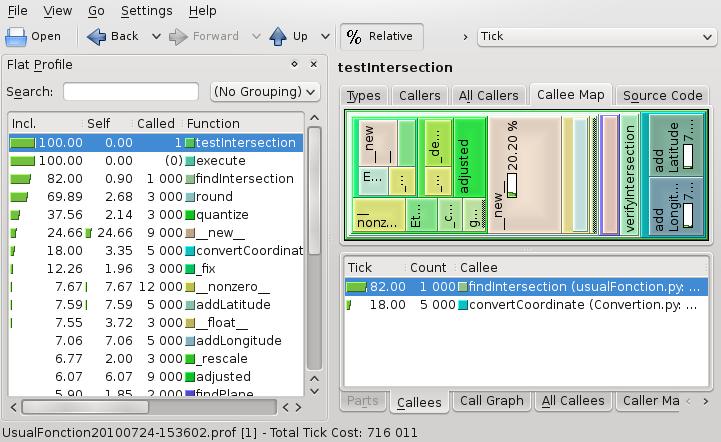
\includegraphics[width=15cm]{images/stats.png}
\caption{Analyse avec Kcachegrind de l'exécution de la fonction "TestIntersection" du programme dans le but de l'améliorer.}
\label{stats}
\end{figure}

Les bottlenecks repérés, une réécriture des parties bloquantes à du être effectuée. Cette analyse nous a permis de réduire les ressources et donc le temps d'exécution du logiciel de plus de 80\%.
